\documentclass{article}
\usepackage{float}
\usepackage{graphicx}

\title{Project 1 - 3SAT generator}
\author{Due June 28, 2017}
\date{}
\begin{document}
\maketitle

%%% Background
\section{Background}
SAT stands for SATisfiability for a given logical expression. That is, given a
logical formula such as $x \wedge y$ are there logical values (TRUE or FALSE)
that can be assigned to $x$ and $y$ to make the whole expression true?

In this case it is clearly the case, simply make $x = $TRUE and $y = $TRUE, but
for more complicated expressions it is not always obvious:
\[
  ((\neg x_1\wedge x_2)\vee x_3) \wedge (\neg x_2 \wedge x_3) \wedge (\neg x_3
  \vee x_2) \wedge (x_1 \vee x_3) \wedge (\neg x_1 \vee (\neg x_2 \wedge x_3))
\]

The goal of a SAT solver is to take an expression as above and determine if some
values for $x_i$ make the whole expression TRUE. Allowing arbitrary logical
expression is very annoying, because of the mixed $\wedge$'s and $\vee$'s. To
fix this there is a standard set. It can be shown that any logical expression
can be written in Conjunctive Normal Form, this process may involve adding extra
``dummy'' values, but will always have the same truth value.

Conjunctive Normal Form (CNF) requires that the expression be separated into
clauses, where each variable is $\vee$'d together and every clause is $\wedge$'d
together. This is complicated to explain but easy to understand through
examples. The above equation is NOT in CNF however the following is, since it is
a collection of clauses (in which variables are only $\vee$'d together) and each
clause is $\wedge$'d together:
\[
  (\neg x_1 \vee x_3 \vee x_4 \vee x_2) \wedge (x_1 \vee \neg x_3) \wedge (\neg
  x_2 \vee \neg x_4)
\]

SAT is a very difficult problem to solve very quickly (in general) it is part of
a class of problems known as NP-Complete.

We will be working with 3SAT, which is a ``simplification''---technically it is
the same problem, but that is above the topics of this course. The
``simplification'' for 3SAT is that each clause must have EXACTLY 3 variables.
So far in this handout we have NOT seen any 3SAT problems. An example of one is:
\[
  (\neg x_5 \vee \neg x_2 \vee x_1) \wedge (x_2 \vee x_5 \vee \neg x_6) \wedge 
  (\neg x_8 \vee x_1 \vee x_3) \wedge (x_9 \vee \neg x_7 \vee x_4)
\]
You'll notice it is perfectly valid to reuse variables between clauses, in fact
if you didn't then this would be very easy to solve.

%%%% Project
\section{Project}
For this project you will be writing a 3SAT generator, that can also test given
truth values. That is, the goal of this program is to create a general 3SAT
problem with at most 10 variables and 10 clauses. Your program will then print
this logical expression so the user can see it (you will use $\sim$ as opposed
to $\neg$) and then ask the user for truth values for each of the variables.
Then it will test whether those truth values make the whole expression TRUE or
not. If they do make the expression TRUE, you should inform the user. If they do
not, you again inform the user AND print the clause which is invalid.

%%%% Expectations
\section{Expectations}
Each run of the program should \emph{randomly} choose the number of possible
variables (between 3 and 10 variables is allowed) it should also \emph{randomly}
choose the number of clauses (between 1 and 10 is allowed). Within a clause, a
variable should not be repeated, ever. That is, $(x_1 \vee x_1 \vee x_2)$ is not
a valid clause, neither is $(x_2\vee \neg x_2 \vee x_3)$. But of course
variables can be repeated between other clauses.

After choosing the number of variables and clauses, each clause should be
generated \emph{randomly}. You may represent this generation anyway that you
like. The standard way to represent a clause is to use a \texttt{list} (in
Python) or an \texttt{int[]} in \texttt{C++}. For example: $(x_1\vee x_2 \vee
x_3)$ can be represented as \texttt{[1,2,3]}, and $(\neg x_2 \vee x_1 \vee \neg
x_5)$ can be represented as \texttt{[-2,1,-5]}, that is, negative numbers
represent a negated variable.

One way to randomly generate clauses is for each clause randomly choose a number
between 1 and the number of variables. This selects your $x_k$, then you should
also randomly decide whether or not to negate this variable, you can do this as
a 50/50 chance.

After \emph{randomly} generating all of the clauses, your program should print
this clause to the screen. Since you cannot directly print $\neg$ you will use
$\sim$ as an alternative. Similarly subscripts are not possible, so you will
just place numbers next to an $x$. You will print something like this:
\[
  (\sim x5 \vee \sim x2 \vee x1) \wedge (x2 \vee x5 \vee \sim x6) \wedge (\sim
  x8 \vee x1 \vee x3) \wedge (x9 \vee \sim x7 \vee x4)
\]
That is, you MUST print parentheses and $\vee$ and $\wedge$, use v and \^{} for
these (it will, ironically, look better printed by your program than by \LaTeX).

After printing the expression you will ask the user for T/F values for each
variable. You MUST ensure input is correct! If I enter: s, (instead of T/F) then
you should ask again until I successfully choose T/F. However you should allow
upper OR lower case, that is, valid inputs are T,t,F,f. Any other inputs are to
be ignored and you should re-ask.

After asking for user input for EVERY variable, you should evaluate whether the
values that were given do or do not satisfy the generated expression. Then you
should inform the user whether they were correct or not, you may use any message
you like to inform the user. But if they were incorrect you MUST also print the
clause that is evaluated to FALSE (and ONLY that clause). It is possible that
many clauses fail, you should print the FIRST clause which fails.

You should not use any external libraries to evaluate the 3SAT expression. There
are many 3SAT solvers in most languages, you should not use these. Programs that
do use them will be penalized, harshly.

Keep in mind the goal of this project is not to solve a 3SAT expression, but to
generate one, and verify a given solution.

%%%% Deliverables
\section{Deliverables}
You need to turn your program into Moodle. You may structure your program
however you desire. Personally I would write this as either 1 Python file or 3
\texttt{C++} files (one \texttt{.h} file, one \texttt{.cpp} file which contains
the implementations of my functions, and one \texttt{.cpp} file which contains
my \texttt{main} method), but as stated do as you please. Moodle will allow only
1 file submission. However you will need to submit a few files, including any
code files and a README file. 

The README file should provide a brief description of your work, describing in
clear English how you solved this project, and any comments you may have for me 
(``I got stuck on this part and could not get it to work'', etc).

Since you need to submit at least 2 files, but are only allowed one file upload,
you will need to create a group of files. I recommend creating a \emph{tarball}.
These are relatively common throughout the programming world, so it may as well
learn it here. \texttt{tar} is a command on Linux which will group files
together with no compression, \texttt{zip} is a command which will compress
files, together they form the \emph{tarball}. On a Linux machine you can create
a \emph{tarball} with the following command:
\[
  \texttt{tar -czvf name-of-archive.tar.gz /path/to/directory-or-file}
\]

%%%% Implementation
\section{Implementation}
Personally, I found this to be easier to write in Python than \texttt{C++}, but
both were very doable. Before beginning to write code you should decide on a
language (obviously) and write down a basic structure. You will find it much
easier to write the code if you write the general structure first. Decide what
functions you want, what you want them to do, then write the code.

You may complete this project in any well known language, that I can easily run
on my Linux system. If you want to choose a slightly less well known language,
talk with me first.

If you choose a language other than \texttt{C/C++}, or Python then you will
receive 5 extra credit points, but will still be held to the same
requirements/standards as others.

%%%%%% Examples
\section{Examples}
The following are examples of my versions of this program running, so that you
can see how the output should be, and how I prompt the user and force correct
input.

\begin{figure}[H]
  \centering
  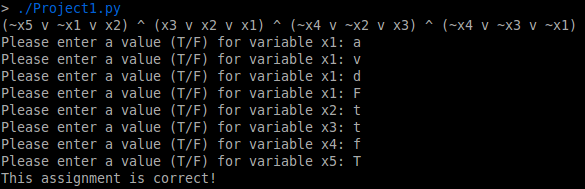
\includegraphics[width=\linewidth]{Ex1}
  \caption{First Example}
  \label{fig:Ex1}
\end{figure}
This example is run with my Python solution, I have made my code executable, you
\emph{should} do this, but it is not required, if you aren't sure how to do
this, you should ask, this is something that you should learn.

In this example we can see I repeatedly ask for input for $x_1$ since the
initial inputs are incorrect. 

\begin{figure}[H]
  \centering
  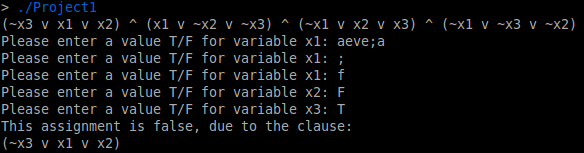
\includegraphics[width=\linewidth]{Ex2}
  \caption{Second Example}
  \label{fig:Ex2}
\end{figure}

This example is my \texttt{C++} solution. 

\begin{figure}[H]
  \centering
  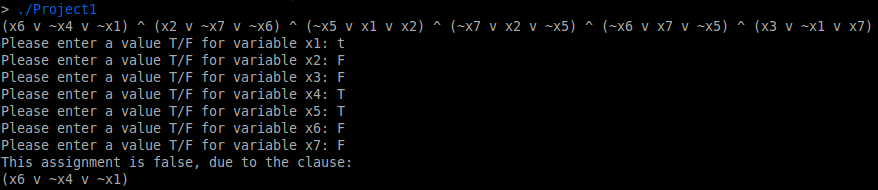
\includegraphics[width=\linewidth]{Ex3}
  \caption{Third Example}
  \label{fig:Ex3}
\end{figure}

Another example of the \texttt{C++} solution.

This picture is a bit smaller due to the long line. You do not need to add extra
newlines to make the output look better, you can but you don't need to. If you
do add artificial newlines the output should look pretty, that is, don't put a
newline in the middle of a clause, do it in between clauses.

%%%% Final Thoughts
\section{Final Thoughts}
Also worthy of note is that since everything is chosen randomly the situation
where you have chosen to use 7 variables but $x_5$ (for example) does not appear
in the randomly generated expression may occur. This is perfectly fine. This
will happen with some non-zero probability based on the number of clauses
there will be. You may decide how to handle this with respect to input
collection. If you choose to still ask the user for a value of $x_5$ that is
fine, if you choose to be clever and skip values that are not used that is also
fine.

Start this project immediately. This project is not conceptually difficult (I
hope!) but there are a lot of details involved. You should start immediately to
run into any issue as soon as possible. If you do run into issues you should be
well aware of the help you can receive. You may work with other students as much
as you would like. HOWEVER you must write your own code. You may talk with
others about the structure of the program. If there is a specific part of the
program you do not how to code you may ask others for examples, but at the end
of the day you must write all of your own code.

You may of course ask me any questions you want and I will be very helpful. This
is expected to be:
\begin{enumerate}
  \item interesting---the 3SAT problem is a very interesting problem.

  \item difficult---handling the details of this program can be very difficult
  to keep straight.

  \item illuminating---hopefully this helps you play with logical expressions
  and gain a deeper understanding. Also determining how to interact with logical
  expressions and strings in a program.
\end{enumerate}
\end{document}
